\documentclass[a4paper,twoside,11pt]{article}
\usepackage[utf8]{inputenc}
\usepackage[english]{babel}
\usepackage{graphicx}
\usepackage{url}
\usepackage{hyperref}
\usepackage{adjustbox}

% pdflatex

% redefinição das margens das páginas
\setlength{\textheight}{24.00cm}
\setlength{\textwidth}{15.50cm}
\setlength{\topmargin}{0.35cm}
\setlength{\headheight}{0cm}
\setlength{\headsep}{0cm}
\setlength{\oddsidemargin}{0.25cm}
\setlength{\evensidemargin}{0.25cm}

\begin{document}

\begin{titlepage}
\begin{center}

% Logo
\resizebox{80mm}{!}{
\includegraphics{../img/logoISEL.png}}

\vspace{1cm}

% Title
{\Large \textbf{Project and Seminar}\\}
\vspace{0.3cm}
{\Large 2024/2025 - 2nd Semester\\}
\vspace{0.8cm}
{\Large Bachelor in Computer Engineering and Informatics\\}
\vspace{1cm}
{\Huge \textbf{Database Documentation}\\}
\vspace{2cm}

% Authors
\begin{tabular}{c}
    Ângelo Azevedo, n.º 50565, e-mail: \href{mailto:a50565@alunos.isel.pt}{a50565@alunos.isel.pt}\\
    António Alves, n.º 50539, e-mail: \href{mailto:a50539@alunos.isel.pt}{a50539@alunos.isel.pt}\\
\end{tabular}

\vspace{2cm}

% Supervisors
\begin{tabular}{ll}
    {Advisor:} & Pedro Matutino, e-mail: \href{mailto:pedro.miguens@isel.pt}{pedro.miguens@isel.pt} \\
    %  & Alberto Caeiro, e-mail: ac@pc.com, PersonCompany\\
\end{tabular}

\vspace{1cm}

March 2025

\end{center}
\end{titlepage}

\section*{Introduction}
The design, development, implementation, and finally, the validation of digital systems require, in addition to simulators, the use of hardware to verify their implementations in real devices. In the current teaching paradigm, in which face-to-face time is reduced and remote and autonomous work is increased, it is necessary to create alternatives to the current model.

The Remote Lab project aims to provide a virtual lab with access to remote hardware. This lab consists of a web application running on an embedded system.
The web application, accessed via a website, aims to provide a dashboard where users can join a laboratory. This is where users can control the remote hardware.
A hierarchy system will be implemented to provide different roles, each with their own permissions relative to how users can browse the information provided by the web application.

\section*{Requirements}
\subsection*{Database}
A database will be used to store the information of the web application.
This includes the user's information, the laboratories' information and the hardware's information.
\begin{itemize}
    \item User information storage
    \item Laboratory configurations and schedules
    \item Hardware specifications and status
\end{itemize}

\subsection*{Web API}
The web API will be a RESTful API that will be used to communicate with the web application.
It will be responsible for the communication with the database and the hardware.
\begin{itemize}
    \item Authentication and authorization endpoints
    \item Laboratory management endpoints
    \item Real-time data communication
\end{itemize}

\subsection*{Authorization}
The authorization will be implemented with a RBAC (Role-Based Access Control) system.
This will allow the user to have different roles with different permissions:
\begin{itemize}
    \item Student
	\begin{itemize}
		\item Enter a laboratory when the professor allows it
		\item Configure, view and control the hardware on the laboratory
		\item Schedule laboratory sessions through the calendar
	\end{itemize}
	\item Professor
	\begin{itemize}
		\item Create, read, update and delete (CRUD) laboratories
		\item Invite students to join the platform through a unique code
		\item Invite students to join a laboratory
		\item See the laboratories' schedules and usage
		\item Create, read, update and delete (CRUD) hardware on the laboratory
	\end{itemize}
	\item Administrator
	\begin{itemize}
		\item Has all the other roles' permissions
		\item Create, read, update and delete (CRUD) users
	\end{itemize}
\end{itemize}

\subsection*{Authentication API}
The authentication API will be a separate RESTful API that will be used to authenticate the user.

\subsection*{Web Application}
The web application will have a dashboard where the user can join a laboratory.
This is where the user can control the remote hardware.
\begin{itemize}
    \item User-friendly interface
    \item Real-time hardware monitoring
    \item Session management
\end{itemize}

\subsection*{Hardware Integration}
There will be a hardware integration module that will be responsible for the integration of the hardware into the web application.

\section*{System Architecture}
The system architecture consists of multiple interconnected components that work together to provide the remote laboratory functionality.
\begin{figure}[h]
	\begin{center}
		\resizebox{16cm}{!}{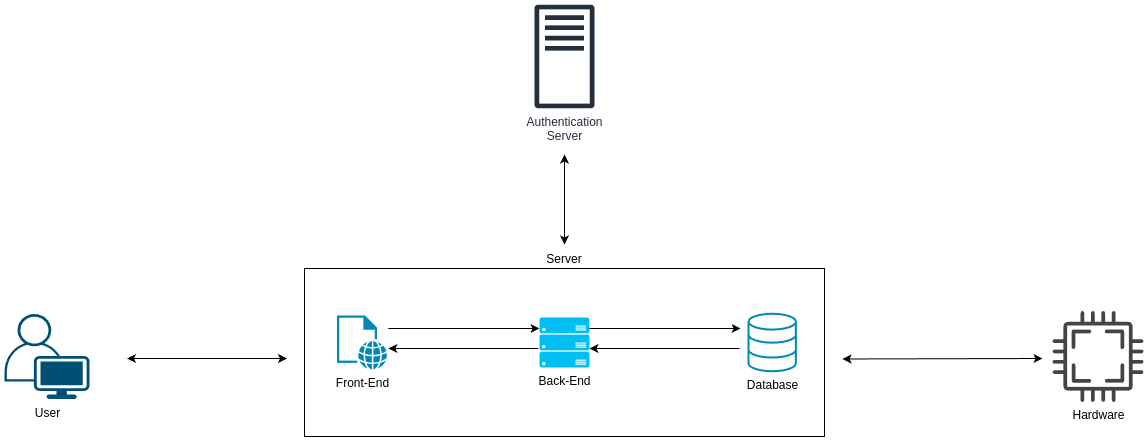
\includegraphics{../img/SystemInfrastracture.drawio.png}}
	\end{center}
	\caption{System Architecture Overview}\label{fig:system-architecture}
\end{figure}

\section*{Timeline}
The project will be developed following the timeline shown in Figure \ref{fig:project-plan}, which outlines the main phases and milestones of the development process.
\begin{figure}[h]
	\begin{center}
		\resizebox{16cm}{!}{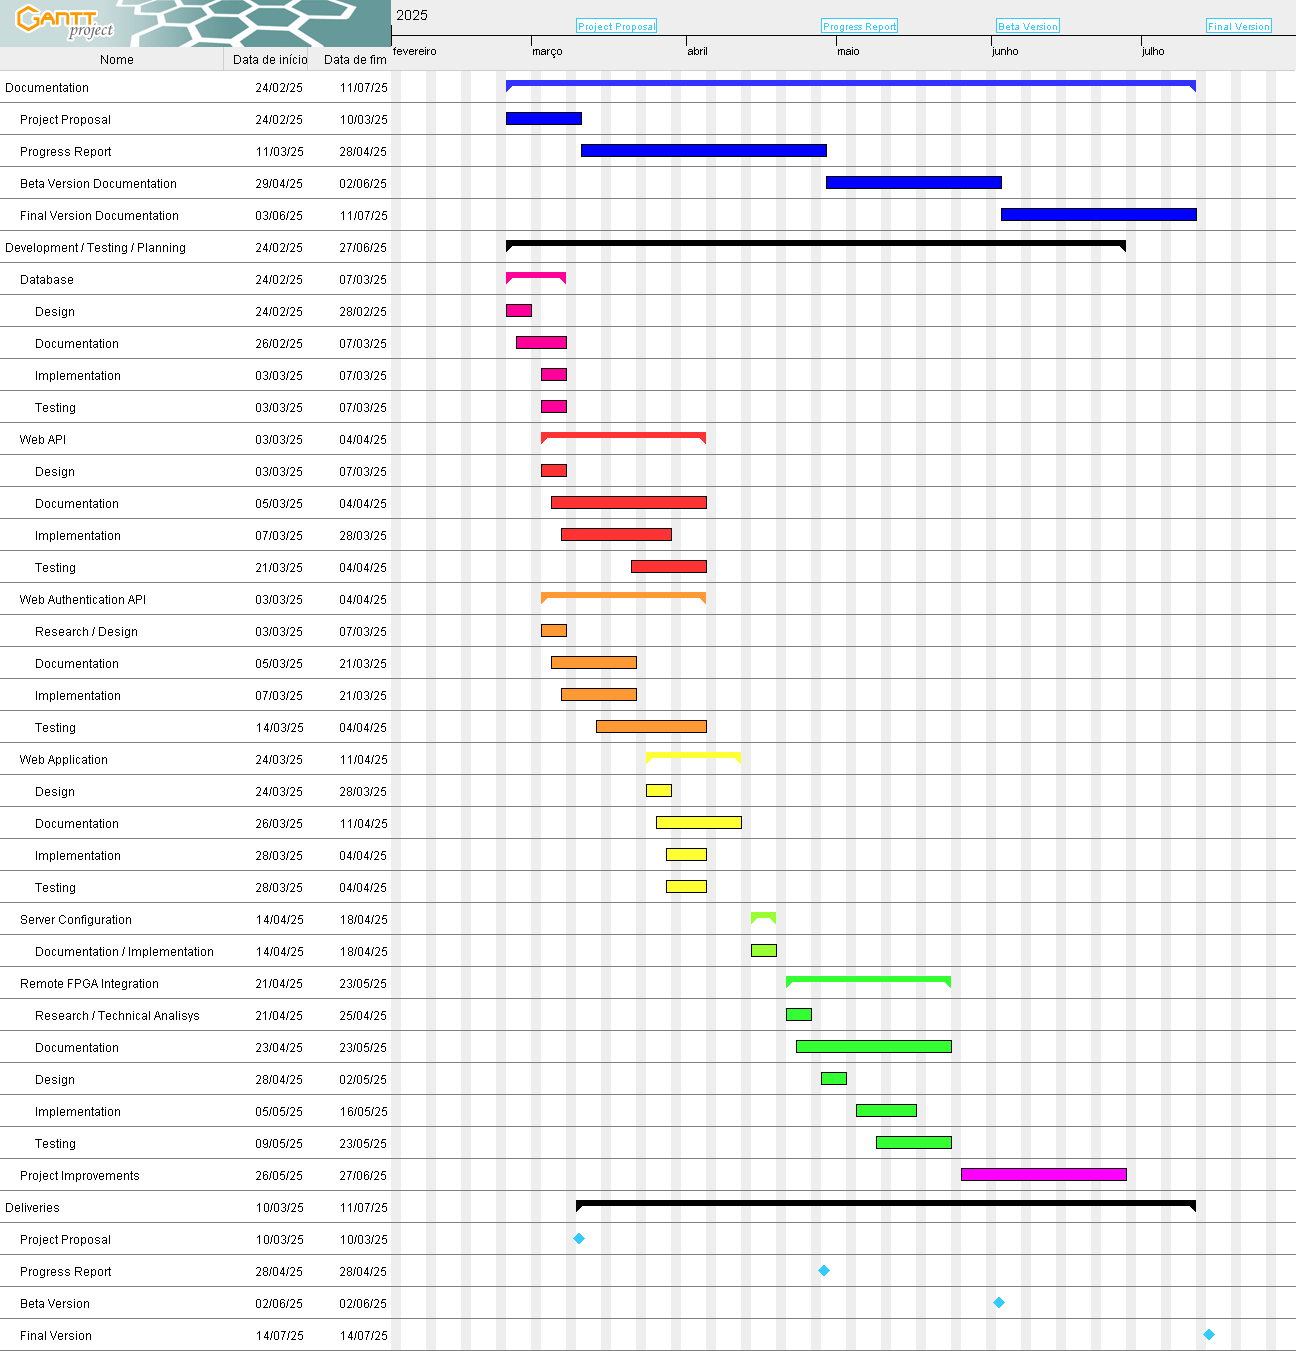
\includegraphics{../img/RemoteLabPlan.png}}
	\end{center}
	\caption{Project Timeline and Milestones}\label{fig:project-plan}
\end{figure}

\end{document}